\documentclass{beamer}
\usepackage{times, amsthm, amsmath, amssymb, cancel, changepage, graphicx, lipsum, fancyhdr, mathabx, enumitem,caption, subcaption}
\usetheme{CambridgeUS}
\usecolortheme{seagull}
\usefonttheme{serif}
\definecolor{navy}{RGB}{0, 0, 128} 
\setbeamercolor{frametitle}{fg=navy}
\setbeamercolor{title}{fg=navy}

\title{\textbf{Lecture 1: Limits and Continuity}}
\date{August 27, 2019}

\begin{document}
	
\frame{\titlepage}

\begin{frame}
\frametitle{\textbf{What is a Limit?}}
We are often interested in values of $f(x)$ of a function $f$ when $x$ is very close to a number $a$, but not necessarily equal to $a$. In many cases $f(a)$ is not defined.
$$\lim\limits_{x \to a} f(x) = L$$
In words: The limit of $f(x)$ as $x$ approaches $a$ is equal to $L$.

\vspace{12pt}

\textbf{Example:}
\begin{itemize}
	\item[(a)] $\lim\limits_{x\to 4} \frac{1}{2}(3x-1)$
	\item[(b)] $\lim\limits_{x\to 9} \frac{x-9}{\sqrt{x}-3}$
	\item[(c)] $\lim\limits_{x\to 2} x^2-x+2$
\end{itemize}
\end{frame}

\begin{frame}
\frametitle{\textbf{Formal Definition of Limit}}
Let $f(x)$ be a function of $x$ defined on some open interval $\mathbb{R}$ that contains a point $a$ except possibly $a$ itself. Then
$$\lim\limits_{x \to a} f(x) = L$$ if and only if for every $\epsilon > 0$ there is $\delta > 0$ such that $|f(x) - L| < \epsilon$ whenever $0 < |x-a| < \delta$.

\vspace{6pt}

\textbf{Some notes:}
\begin{itemize}
	\item[1.] $f(x)$ does not have to equal $L$ for the limit to exist.
	\item[2.] Examine the behavior of $f(x)$ as $x \to \infty$.
	\item[3.] The limit does not have to exist.
\end{itemize}

\vspace{6pt}

\textbf{Example:}
\begin{itemize}
	\item[(a)] Show $\lim\limits_{x \to 0} x^2=0$
\end{itemize}
\end{frame}

\begin{frame}
\frametitle{\textbf{One-sided Limits}}
We can examine the limit as $x$ approaches from the left or right. This is called a one-sided limit.
\begin{eqnarray*}
\mbox{Left-handed limit}: & \lim\limits_{x \to a^-} f(x) = L^-\\
\mbox{Right-handed limit}: & \lim\limits_{x \to a^+} f(x) = L^+\\
\end{eqnarray*}
For the limit to exist $L^- = L^+ = L$

\vspace{12pt}

\textbf{Example:}
\begin{itemize}
\item[(a)]
$f(x)=  \begin{cases} 
0 & \mbox{ for } x <0\\
1 & \mbox{ for } x \geq 0
\end{cases}  $
\end{itemize}
\end{frame}

\begin{frame}
\frametitle{\textbf{Limit Laws}}
Suppose $c$ is a constant, $n$ is a positive integer, and $\lim\limits_{x \to a}f(x)$ and $\lim\limits_{x \to a}g(x)$ exist.
\begin{itemize}
	\item[1.] $\lim\limits_{x \to a} [f(x)+g(x)] = \lim\limits_{x \to a}f(x) + \lim\limits_{x \to a}g(x)$
	\item[2.] $\lim\limits_{x \to a} [f(x)-g(x)] = \lim\limits_{x \to a}f(x) - \lim\limits_{x \to a}g(x)$
	\item[3.]$\lim\limits_{x \to a}[cf(x)] = c\lim\limits_{x \to a}f(x)$
	\item[4.]$\lim\limits_{x \to a}[f(x)g(x)] = \lim\limits_{x \to a}f(x)\lim\limits_{x \to a}g(x)$
	\item[5.]$\lim\limits_{x \to a}\frac{f(x)}{G(X)} = \frac{\lim\limits_{x \to a}f(x)}{\lim\limits_{x \to a}g(x)} \mbox{ if } \lim\limits_{x \to a} g(x) \neq 0$
	\item[6.]$\lim\limits_{x \to a}[f(x)]^n = [\lim\limits_{x \to a}f(x)]^n$
\end{itemize}
\end{frame}

\begin{frame}
\frametitle{\textbf{Limit Laws}}

\begin{itemize}
	\item[7.]$\lim\limits_{x \to a}c=c$
	\item[8.]$\lim\limits_{x \to a}x=a$
	\item[9.]$\lim\limits_{x \to a}x^n = a^n$
	\item[10.]$\lim\limits_{x \to a} \sqrt[n]{x} = \sqrt[n]{a}$
	\item[11.]$\lim\limits_{x \to a} \sqrt[n]{f(x)} = \sqrt[n]{\lim\limits_{x \to a} f(x)}$
\end{itemize}

\vspace{12pt}

\textbf{Examples:}
\begin{itemize}
	\item[(a)] Find $\lim\limits_{x \to 2}\frac{3x+4}{5x+7}$
	\item[(b)] Show that for every real number $a$, $\lim\limits_{x \to a}x^3=a^3$
	\item[(c)] Find $\lim\limits_{x \to 2}(3x+4)^5$
\end{itemize}
\end{frame}

\begin{frame}
\frametitle{\textbf{Continuity}}
A function is continuous at a number $a$ if $\lim\limits_{x \to a}f(x)=f(a)$. This definition requires that:
\begin{itemize}
	\item[1.] $f(a)$ is defined
	\item[2.]$\lim\limits_{x \to a}f(x)$ exists.
	\item[3.]$\lim\limits_{x \to a}f(x)=f(a)$
\end{itemize}
A continuous function has the property that a small change in $x$ produces only a small change in $f(x)$.

\vspace{12pt}

\textbf{Example:}
\begin{itemize}
	\item[(a)] Is $f(x) = \frac{x^2-x+2}{x-2}$ continuous at $8$ and $4$?
\end{itemize}
\end{frame}

\begin{frame}
\frametitle{\textbf{Types of Continuity}}
\textbf{Left \& Right Continuity}

We can examine the continuity of a function from either the left or the right.
\begin{eqnarray*}
	\mbox{Left continuous}: & \lim\limits_{x \to a^-} f(x) = f(a)\\
	\mbox{Right continuous}: & \lim\limits_{x \to a^+} f(x) = f(a)\\
\end{eqnarray*}$f$ is continuous if and only if $f$ is continuous from the left and right at every point in its domain.
\vspace{12pt}

\textbf{Interval Continuity}

$f$ is continuous on $[a,b]$ if it is continuous on every point on the interval

\vspace{12pt}

\textbf{Example:}
\begin{itemize}
	\item[(a)] Show that $f(x) = 1-\sqrt{1-x^2}$ is continuous on $[-1,1]$
\end{itemize}
\end{frame}

%\begin{frame}
%\frametitle{What is a Limit?}
%\begin{figure}
%	\centering
%	\begin{subfigure}{0.48\textwidth}
%		
%		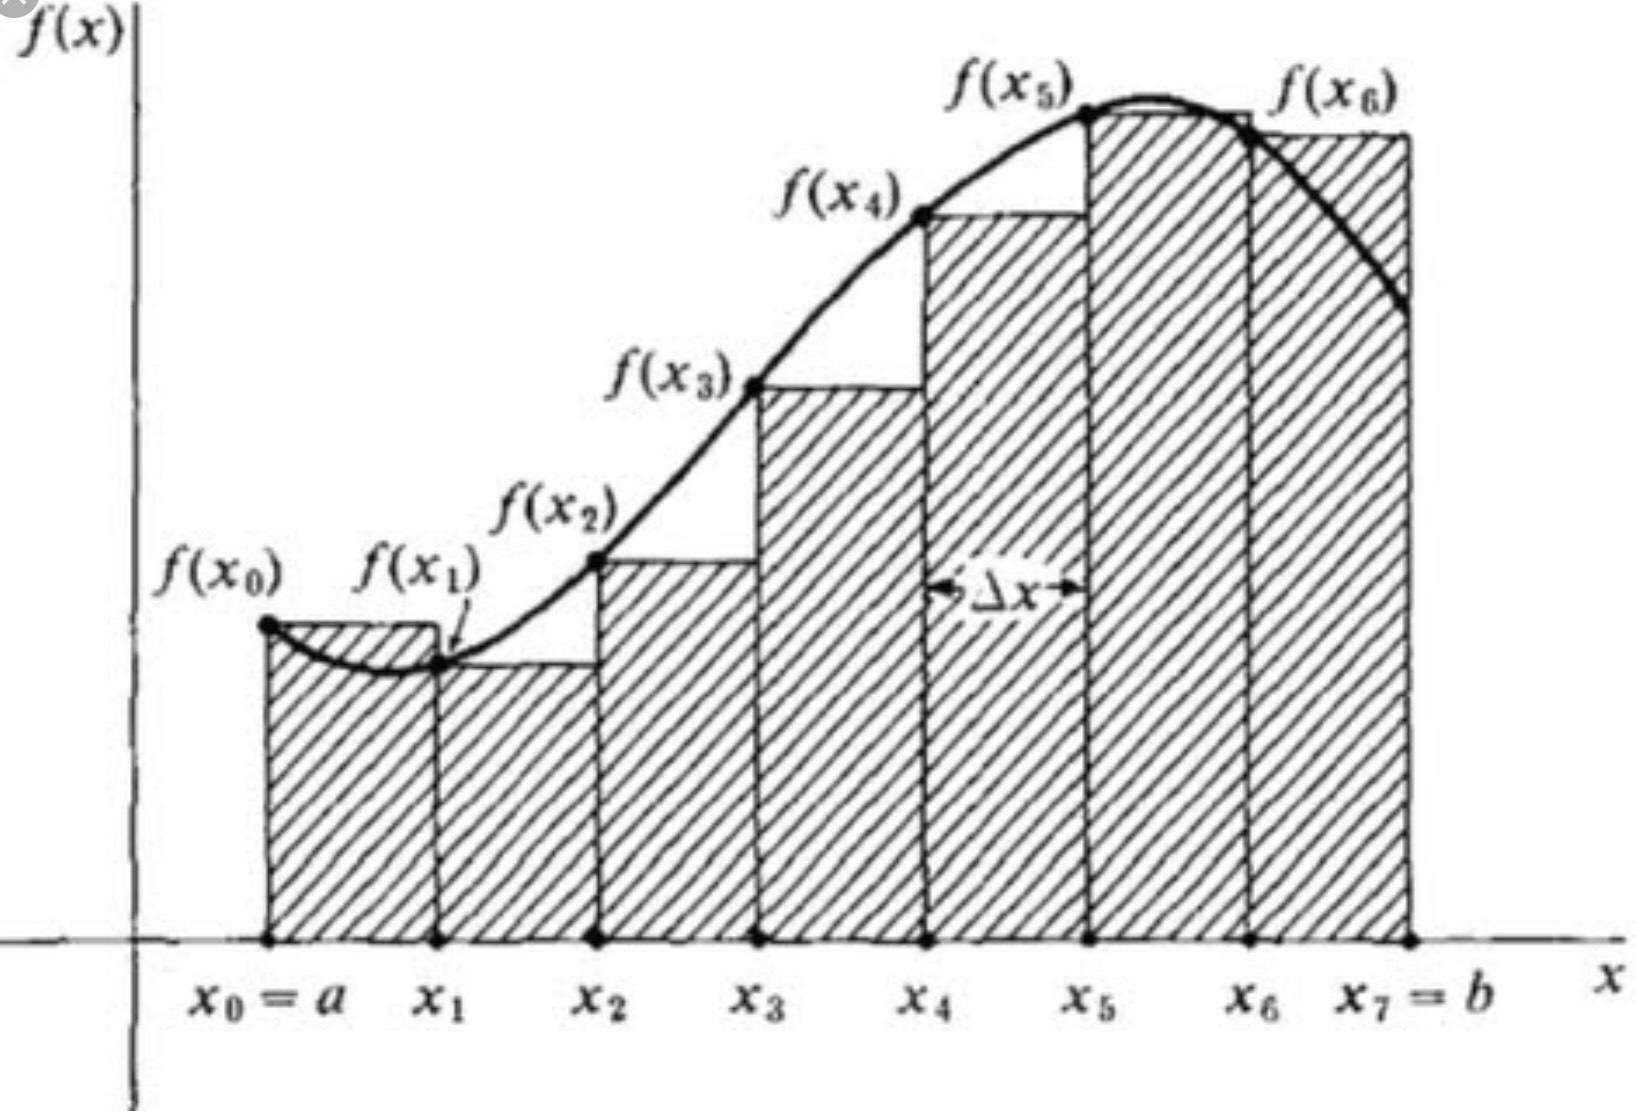
\includegraphics[width=\textwidth]{IMG_0380.jpg}
%		\hspace*{10pt}\hbox{\thinspace{\tiny\itshape vias.org}}
%		\caption{Single integration}
%	\end{subfigure}% 
%	~ 
%	\begin{subfigure}{0.48\textwidth}
%		
%		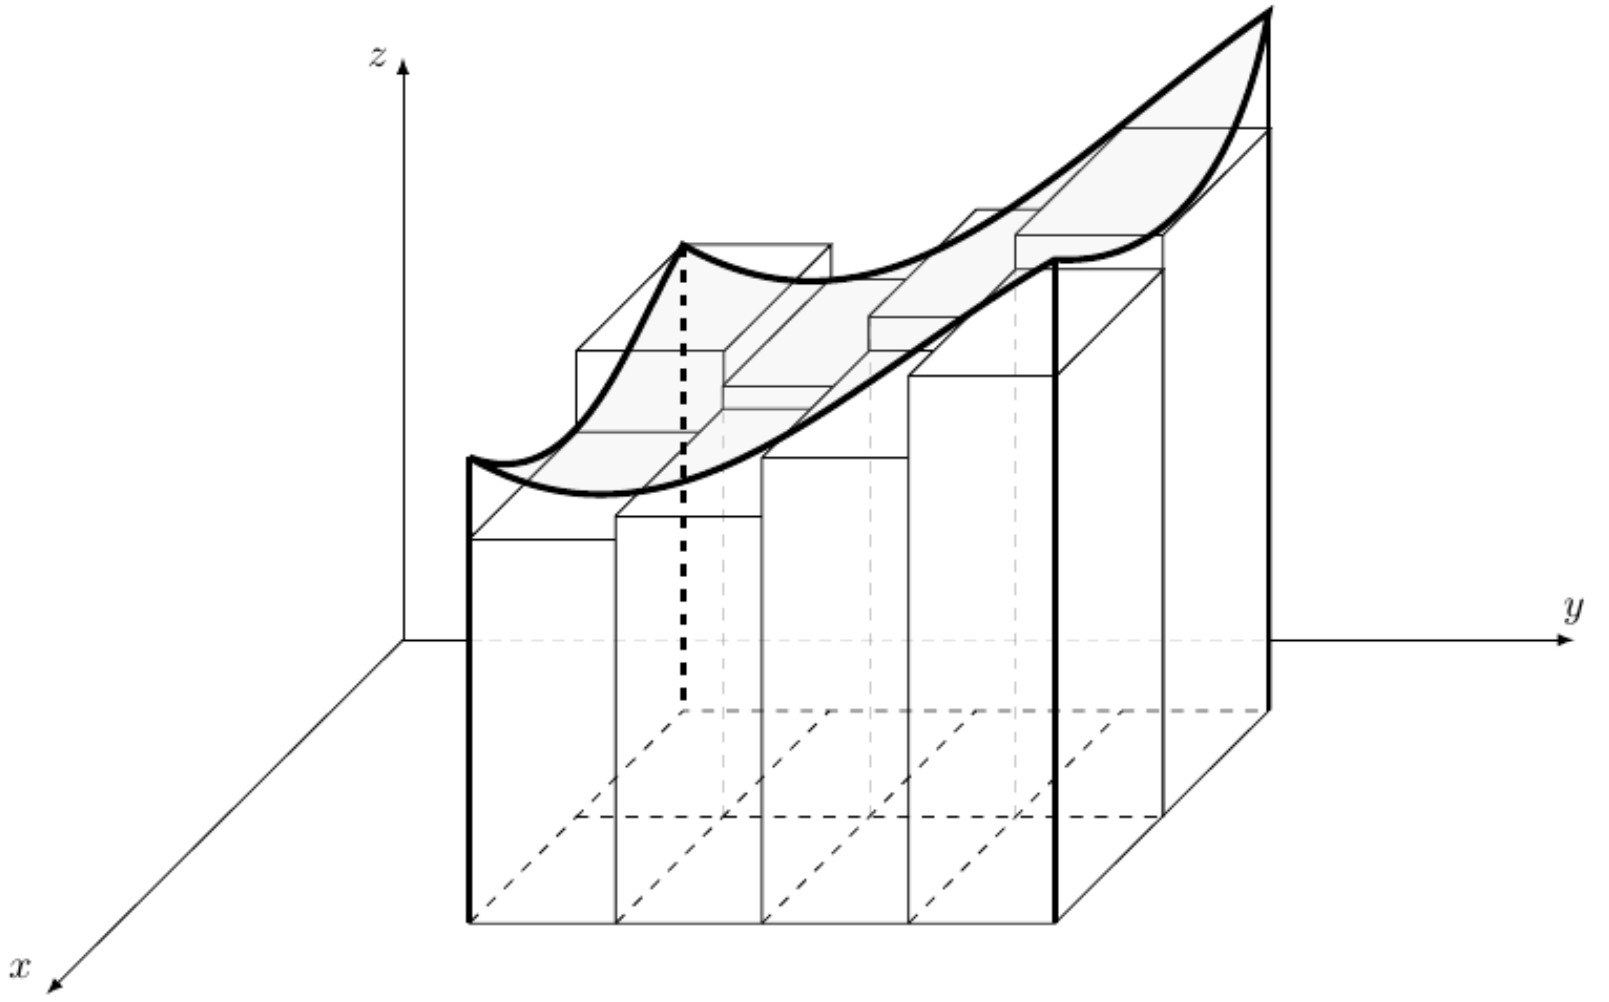
\includegraphics[width=\textwidth]{IMG_0385.jpg}
%		\hspace*{10pt}\hbox{\thinspace{\tiny\itshape tex.stackexchange.com}}
%		\caption{Double integration.}
%		\label{fig:2}
%	\end{subfigure}
%\end{figure}
%
%\end{frame}
%
%
%\begin{frame}
%\frametitle{Triple Integral}
%\begin{figure}
%	\centering
%	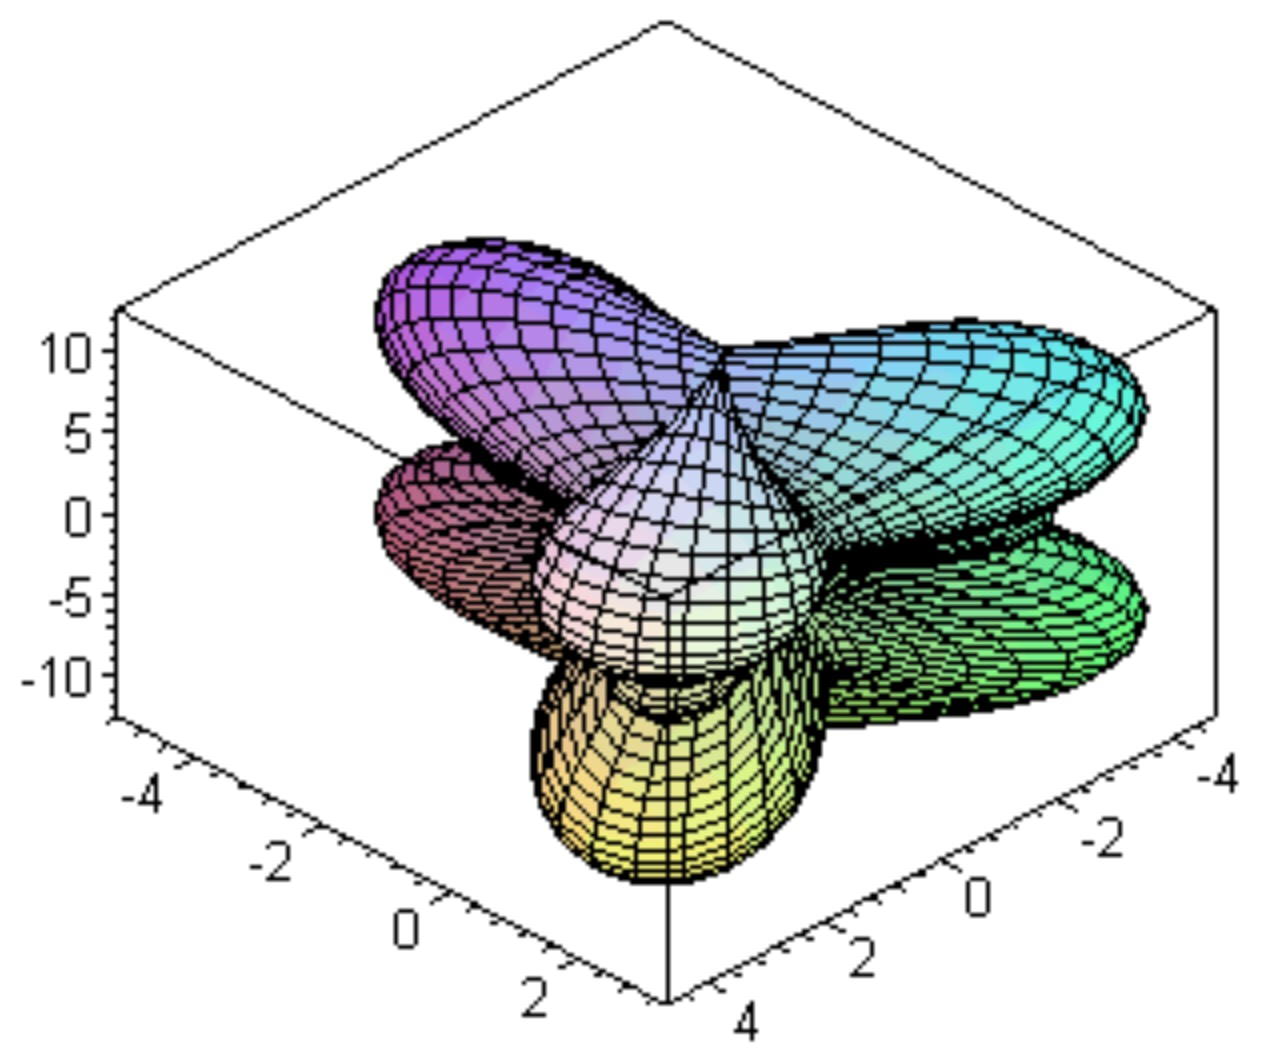
\includegraphics[height=.45\textheight]{IMG_0384.jpg}\\
%	\hspace*{10pt}\hbox{\thinspace{\tiny\itshape maplesoft.com}}
%\end{figure}
%
%$$\iiint\limits_{\mathbb{R}} F(x,y,z) dV = \int_{x=a}^{x=b} \int_{y=y_1(x)}^{y=y_2(x)} \int_{z=z_1(x,y)}^{z=z_2(x,y)} F(x,y,z) dz\,dy\,dx$$
%\textbf{Example:}
%\begin{itemize}
%	\item[(a)] $\int_0^1 \int_0^{1-x} \int_0^{2-x} xyz \,dz\,dy\,dx$
%\end{itemize}
%\end{frame}

\end{document}
